\documentclass[/Users/ikedahajime/GitHub/reserch/master_report/thesis]{subfiles}
% このファイル内だけのコマンド
\begin{document}
\chapter{結果}
\section{壁の形状による影響}
この章では、壁の形状を変えたときの結果を示す。具体的には、壁の形状を1つの円から2つの円をつなげたものに変え、そのダイナミクスを見る。
TODO:ここに粒子はいち
\begin{figure}[htbp]
    \centering
    \begin{tabular}{c}
        \begin{minipage}{0.3\hsize}
            \text{(a)}
            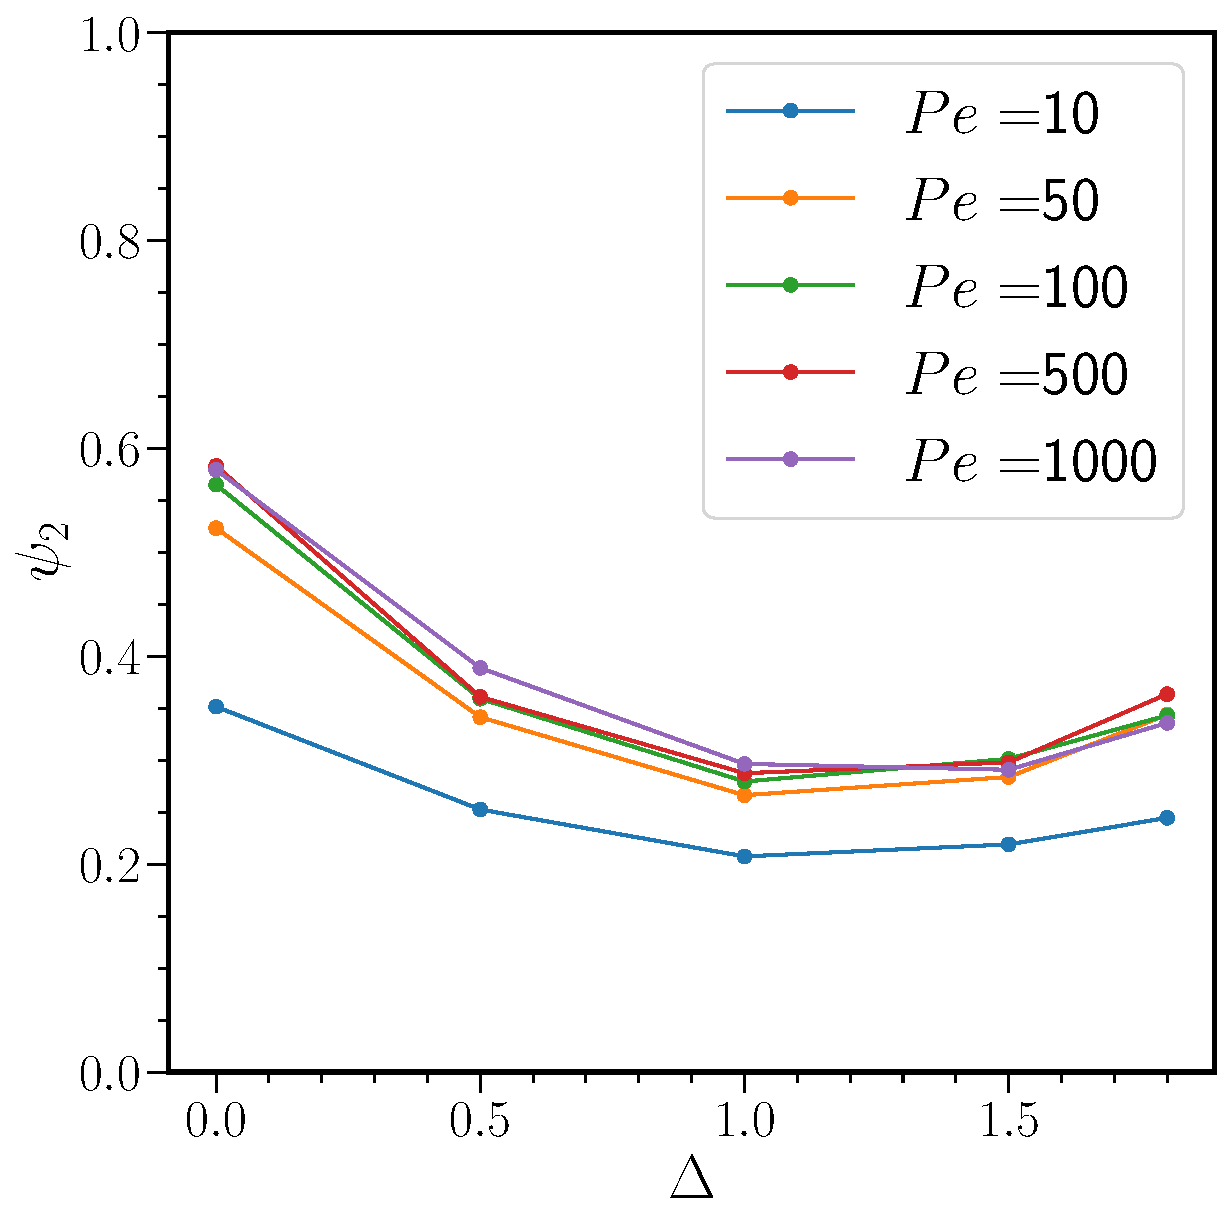
\includegraphics[width=\textwidth]{img/bit/ani_test/psi_20.70.110.pdf}
        \end{minipage}
        \begin{minipage}{0.3\hsize}
            \text{(b)}
            \includegraphics[width=\textwidth]{img/bit/ani_test/L_{z2}0.70.110.pdf}
        \end{minipage}
        \begin{minipage}{0.3\hsize}
            \text{(c)}
            \includegraphics[width=\textwidth]{img/bit/ani_test/V_{2}0.70.110.pdf}
        \end{minipage}
    \end{tabular}
    \caption[two_hdlm]
    {
        $\varphi=0.7、R=10、M=0.1$
    }
    \label{fig:twocer_lo0.7_r10_m0.1}
\end{figure}
%時間依存性
% 全体の華香
% 何を言う?
\end{document}
